\chapter{Prototype: Live Data Simulation} \label{sec:simulationprototype}

\section{Purpose}

The previous chapter identified that the best way to implement a Digital Twin system is to implement an adapter, or bridging system, between the simulation platform and the factory SCADA system. This chapter describes a prototype of an adapter layer.
This prototype is developed for demonstration purposes, illustrating how the Ahuora Simulation Platform could be integrated with a real-time data processing system. As such, this prototype reflects a minimum-viable product, assessing the feasibility of the architecture developed in the research stage. Insights from the prototype are used to refine the requirements of subsequent work.

\section{Method}

\begin{wrapfigure}{r}{0.5\textwidth}
    \centering
    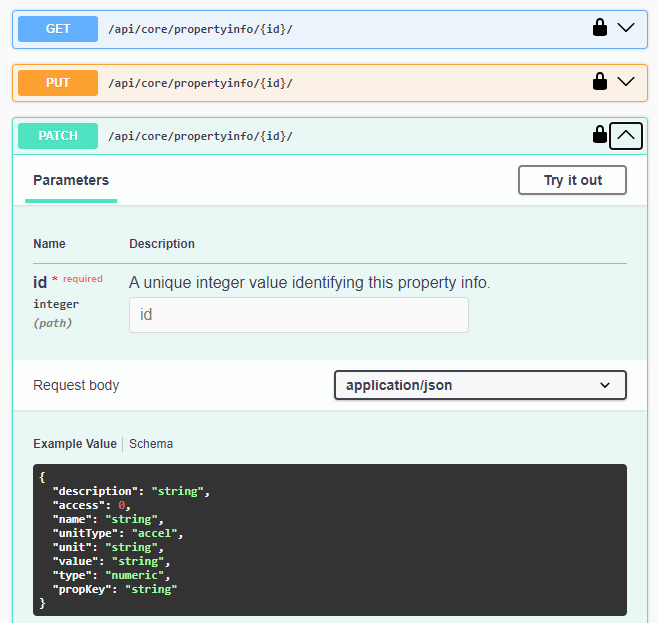
\includegraphics[width=0.5\textwidth]{swaggerprops.png}
    \caption{Swagger definition of API endpoints for updating properties.}
    \label{fig:swaggerendpoints}
\end{wrapfigure}

The Ahuora Simulation Platform has a REST API that is used internally to communicate between the frontend and the backend. This API already includes endpoints for updating properties, and retrieving properties after a simulation. This API could also be used for real-time data processing systems to communicate programmatically with the platform.

The flowsheet needs to be set up ahead of time with the relevant unit operations, and properties. Each property field has a unique ID, generated by the database. To solve the flowsheet repeatedly based on real-time data, the properties in the flowsheet are updated programmatically to reflect the real-time state of the system. Following this, a call is made to the API endpoint to solve the flowsheet. Relevant properties can then be queried to get the results of the simulation.

\begin{figure}
    \centering
    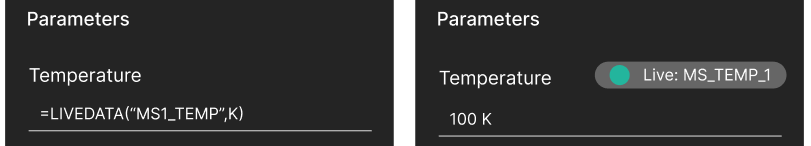
\includegraphics[width=0.8\textwidth]{property_ui.png}
    \caption{Prototype UI designs for setting a property as a ``real-time'' property.}
    \label{fig:property-ui}
\end{figure}

As the property IDs are generated by the database, it does not make sense to hard-code them into the real-time data processing system. Rather, a more generic way of referring to properties that need to be updated is required. 
Some prototyping of a UI method to set properties as ``real-time'' in the existing interface was done, as shown in \Cref{fig:property-ui}. 
This allows the user to select which properties should be updated in real-time, and establishes a mechanism to refer to such properties within the real-time data processing system. 
The work within this project stopped short of implementing full real-time data integration. This decision was made in part because there is not yet a clear delineation between the workflows of an engineer and a plant operator within the Ahuora Simulation Platform. Furthermore, for the purposes of a proof of concept implementation required within the scope of this work, simulating live inputs from dummy data was considered adequate.

A simple definitions file was used to map the properties in the Ahuora Simulation Platform to the properties in the simulated real-time data processing system. 
As shown in \Cref{fig:live-constants}, the file included the unit operation name, the property key (used by the Ahuora Simulation Platform to determine property types), and the sensor ID from the real-time data processing system. 
The data processing platform could use this information to find the property IDs in the Ahuora Simulation Platform, and update them with the real-time data.

\begin{figure}
    \centering
    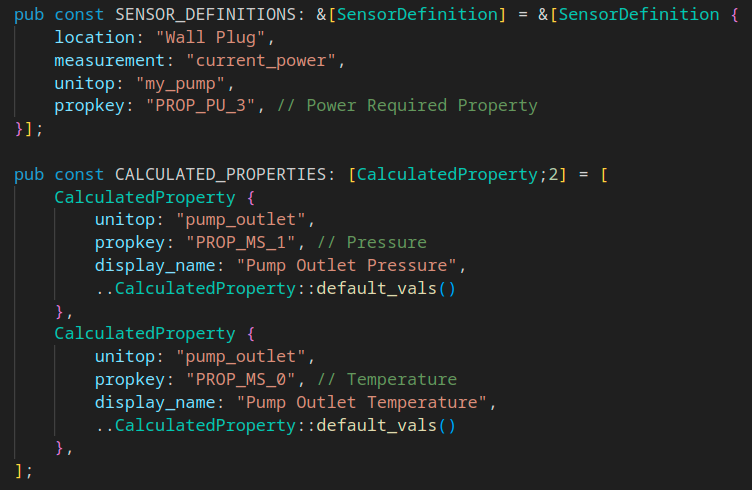
\includegraphics[width=0.8\textwidth]{live_constants.png}
    \caption{Definitions file for mapping properties in the Ahuora Simulation Platform to the real-time data processing system.}
    \label{fig:live-constants}
\end{figure}

Simulation of real-time data was achieved through the use of CSV file with dummy data points.  
This approach was appropriate for development purposes within the scope of a proof of concept prototype, as functional changes and debugging were able to be undertaken in a rapid fashion without being limited by time constraints associated with restarting a physical system. It is worth noting that the format of this data was consistent with historic data recorded from real-time sensors collected in \Cref{sec:heatpumpcollection}. Therefore it is reasonable to extrapolate that the success of the implemented solution across multiple timesteps defined within the dummy data is demonstrable of the potential of the prototyped approach for live data situations.

This prototype also used a very simple model: a pump with an inlet stream and an outlet stream. 
The power used by the pump was calculated based on the  ``live'' data, and the inlet streams were already specified. 
The simulation was used to calculate the outlet pressure and temperature of the pump. This is a simple model, but it is sufficient to demonstrate the feasibility of the architecture.

% TODO: Add image: Running the simulation on the CSV file.

When the script file was run, for each new data point, the script updated the properties in the Ahuora Simulation Platform, and then called the API to solve the simulation. The results of the simulation were then printed to the console. 

This worked suprisingly well, and was able to be done in only around 300 lines of code. 
It was implemented in Rust, using an API client SDK generated from the OpenAPI specification of the Ahuora Simulation Platform. 
This made it fully type-safe and reliable. 
Because of the configuration file format, it is trivial to add a longer list of sensors and calculated properties, as is required in more complex properties.

\section{Discussion} \label{sec:prototypeinsights}

This prototype demonstrated that the Ahuora Simulation Platform can be integrated with a real-time data processing system with relatively little effort, as long as there is a standardised API. 
Depending on the type and quality of the sensor data, there may need to be some data cleaning and preprocessing, specific to a particular use case. 
Hence, any data preprocessing pipeline or service for the Ahuora Digital Twin Platform should be kept as simple as possible.
To confirm this, the heat pump dryer was then used as a case study in linking a more complex system to the Ahuora Simulation Platform. 
This provides a more realistic test of the architecture.

This approach, which closely follows the architecture described in \Cref{fig:architecture} in \Cref{sec:researchconclusions}, also outsources the processing, visualisation, and control actions to third-party systems, as all data would be stored in the factory's existing knowledge base after processing, completely external to all Ahuora Systems. The only data that the Ahuora Digital Twin Platform would need to store is the current state of the system. 

This makes it easier to build a ``headless" version of the Ahuora Simulation platform that can be deployed as a single frozen model, into a factory's existing systems. 
This is beneficial for stability and reliability reasons, limiting the complexity of the system. This is the unix ``do one thing and do it well" philosophy applied to software architecture.

% TODO: THis needs to be reworked

However, there are disadvantages to this approach. 
One of the key value propositions of the Ahuora Digital Twin Platform is that it provides one place to define a factory's architecture, and then multiple types of analysis can be used on it. The same structures could be helpful for automatically creating visualisations of the real-time state of the factory, fault diagnostics, control, and surrogate modelling. 
As the platform currently stands, it cannot be considered a ``Digital Twin'', as true digital twins include multiple fidelities of simulation, and dynamic ``state'' that adapts to real-world conditions via a feedback loop. 
The next steps in development will need to balance these two approaches, to find an architecture that includes the advantages of each.
